\chapter{ParVis}
\section{Introduzione}
In questo capitolo illustremo ParVis, un tool grafico che viene utilizzato per rappresentare graficamente le operazioni che vengono effettuate dai parser. Questo tool offre la possibilità di illustrare graficamente le strutture dati usate dal parser, l'albero sintattico, il testo in input su cui si sta facendo il parsing, il simbolo e lo stato corrente che si sta analizzando. Nei paragrafi successivi illustreremo le componenti basi utilizzate da ParVis, il suo funzionamento e le componenti create per rappresentare graficamente il GLL Parsing.
\section{Il prompt dei comandi}
Il \textbf{prompt dei comandi} è la componente fondamentale che viene usata per gestire le impostazioni grafiche di ParVis, l'esecuzione e il caricamento delle operazioni da illustrare. Per avviare l'esecuzione di un illustrazione grafica è necessario caricare il file \textbf{\textit{log.json}}. Questo file viene generato dopo l'esecuzione del parser e contiene le operazioni di log effettuate. Nella figura 7.1 viene illustrato il prompt dei comandi. Presenta un menu "File" e "Windows" che sono utilizzati, rispettivamente, per caricare il file \textit{log.json} e per settare le impostazioni grafiche delle finestre. Poi vi sono tre pulsanti dove i primi due, a partire da sinistra, sono utilizzati per eseguire un operazione in avanti e all'indietro; mentre il terzo viene usato per automatizzare l'esecuzione delle operazioni. Nella parte principale del prompt dei comandi è presente una lista che contiene i vari item delle produzioni, chiamati \textbf{stati}. Questi stati sono raccolti in menu a tendina poichè contengono le varie operazioni effettuate per gestire un item. Possono essere aperti e chiusi cliccando o su singolo stato o con i pulsanti in alto alla lista. Uno stato evidenziato indica che ParVis sta visualizzando le operazioni di quello stato, se lo si apre vedremo evidenziate le sue operazioni all'interno. In basso alla lista è presente uno slider che viene utilizzato per eseguire più velocemente le operazioni di visualizzazione.\par
\begin{figure}[hbpb]\label{prompt}
	{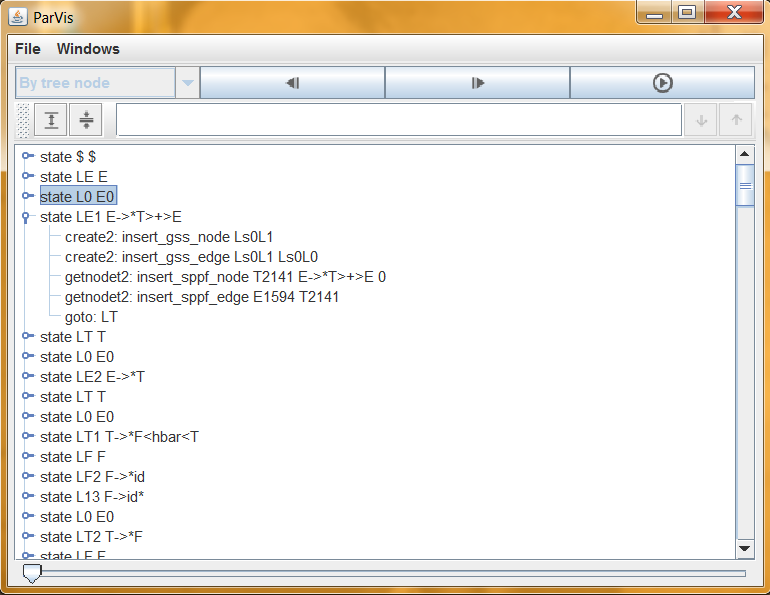
\includegraphics[height=350pt,width=420pt,scale=0.1]{files/ParVisCommand.png}}
	\caption{\textit{Prompt dei comandi}}
\end{figure}
\section{Le componenti grafiche del GLL Parsing}
In questo paragrafo verranno illustrate le componenti grafiche realizzate per il GLL Parsing. Queste componenti sono state implementate nel file \textbf{\textit{jsonreader.js}} e ne sono state definite le impostazioni grafiche. Ogni finestra presenta un toolitip in cui vengono descritte le informazioni contenute da ogni elemento grafico. Ogni finestra subisce continue modifiche per ogni operazione che si sta eseguendo.\par
\begin{figure}[hbpb]\label{insiemeU}
	\centering
	{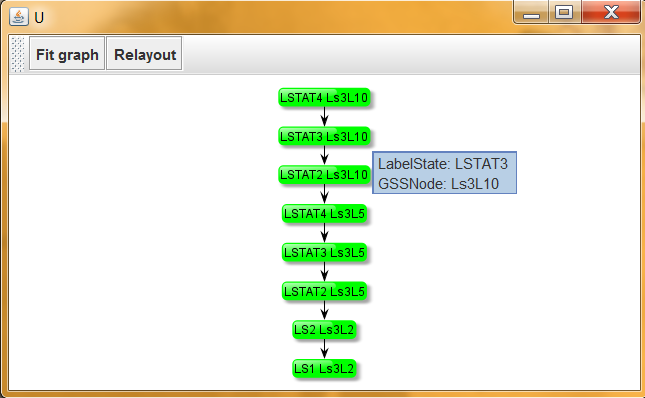
\includegraphics[height=200pt,width=320pt,scale=0.1]{files/InsiemeU.png}}
	\caption{\textit{Insieme U}}
\end{figure}
\noindent L'insieme U (fig. 7.2) viene rappresentato come una lista di nodi collegati uno dietro l'altro. Riporta le seguenti informazioni: il nome dello stato e il nome del nodo del GSS.\par
\begin{figure}[h]\label{input}
	\centering
	{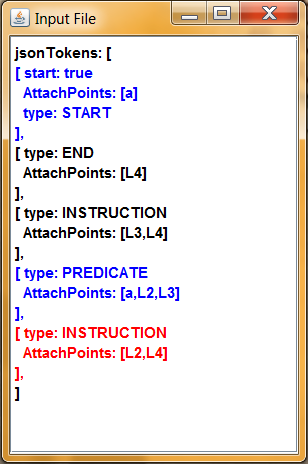
\includegraphics[height=180pt,width=120pt,scale=0.1]{files/Input.png}}
	\caption{\textit{Testo in Input}}
\end{figure}
\noindent L'input (fig. 7.3) viene rappresentato allo stesso modo in cui è stato definito nel file d'input. Sull'input vengono utilizzati tre colori: il nero indica un simbolo non ancora letto, il rosso indica un simbolo che il parser vuole trovare ed il blu indica un simbolo che è stato trovato dal parser.\par
\begin{figure}[hbpb]\label{insiemeP}
	\centering
	{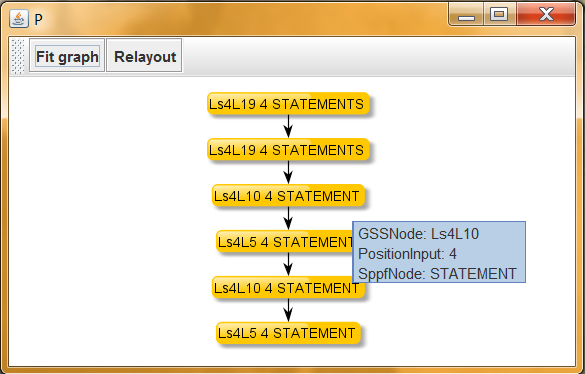
\includegraphics[height=190pt,width=320pt,scale=0.1]{files/InsiemeP.png}}
	\caption{\textit{Insieme P}}
\end{figure}
\noindent L'insieme P (fig. 7.4) è rappresentato come una lista di nodi. Sono state rappresentate le seguenti informazioni: il nodo del GSS, la posizione del simbolo da trovare e il nodo dell'SPPF.\par
\begin{figure}[hbpb]\label{gss}
	\centering
	{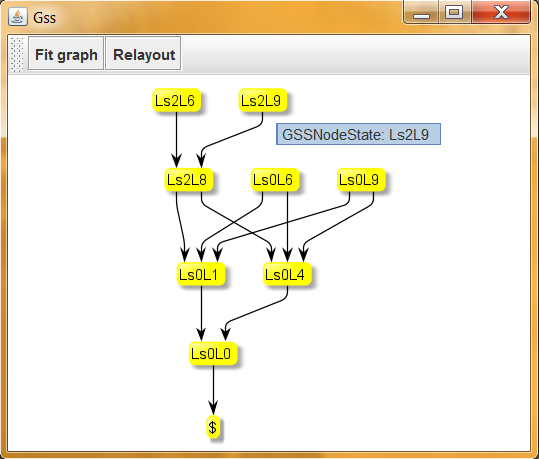
\includegraphics[height=190pt,width=250pt,scale=0.1]{files/GSS.png}}
	\caption{\textit{GSS}}
\end{figure}
\noindent La figura 7.5 mostra la rappresentazione grafica del GSS. Viene rappresentato come un grafo diretto aciclico (DAG) che non contiene cicli. Ogni nodo contiene le informazioni sul simbolo che si vuole trovare e lo stato che identifica l'item da processare. Il loro nome viene rappresentato in base alle notazioni descritte al capitolo 5.\par
\begin{figure}[hbpb]\label{SPPF}
	{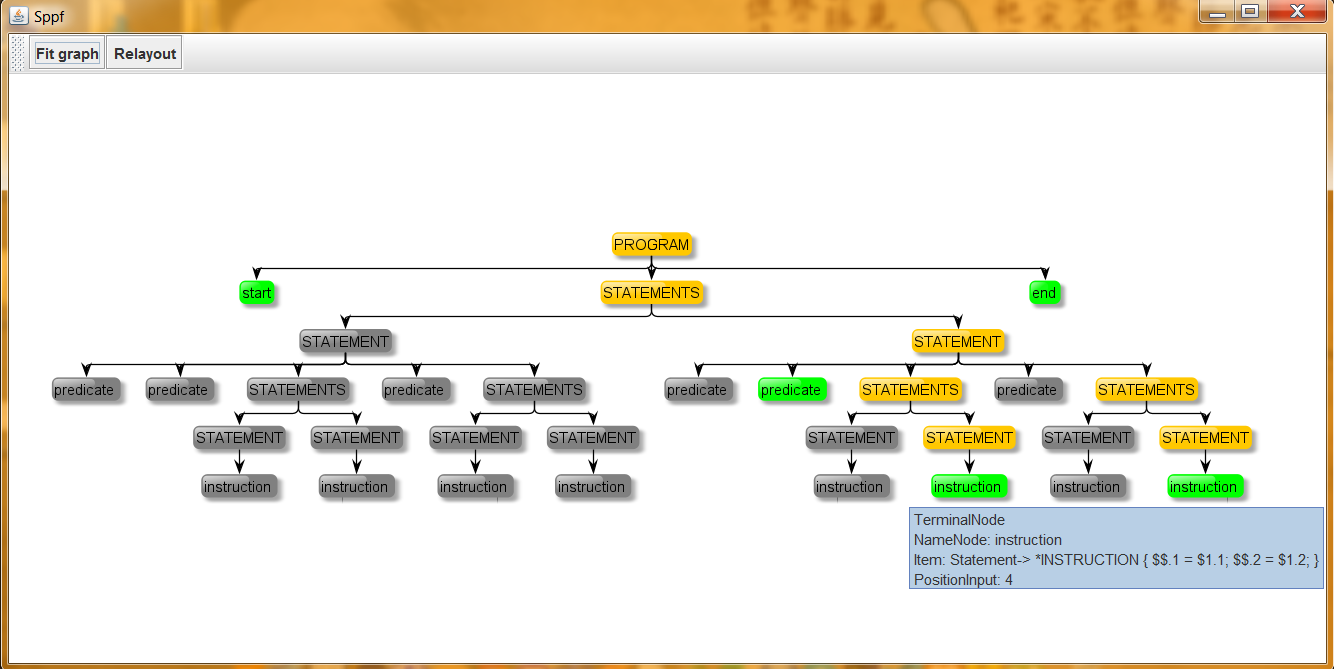
\includegraphics[height=260pt,width=420pt,scale=0.1]{files/SPPF.png}}
	\caption{\textit{SPPF}}
\end{figure}
\noindent L'SPPF (fig. 7.6) viene rappresentato con vari tipi di nodi: i nodi arancioni vengono usati per identificare i non-terminali, i nodi verdi vengono usati per i terminali, i nodi grigi rappresentano tutti quei nodi che appartengono a produzioni che non sono state completate per intero, nel tooltip vengono segnati come \textit{Not Valid}. Le informazioni riportate sono: il tipo del nodo, la posizione che occupa nell'input (solo per i terminali), il nome del simbolo, l'item di produzione a cui appartiene.\par 
\begin{figure}[hbpb]\label{currentState}
	\centering
	{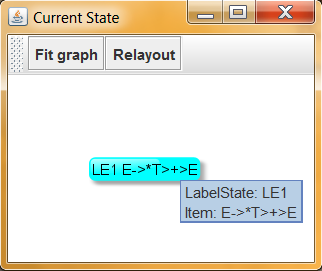
\includegraphics[height=110pt,width=110pt,scale=0.1]{files/CurrentState.png}}
	\caption{\textit{Stato Corrente}}
\end{figure}
\noindent La finestra in figura 7.7 viene utilizzata per rappresentare lo stato corrente su cui il parser sta eseguendo le operazioni. \'E composta da un nodo che indica il nome dello stato e l'item che sta processando.\par
\begin{figure}[hbpb]\label{DumpFile}
	\centering
	{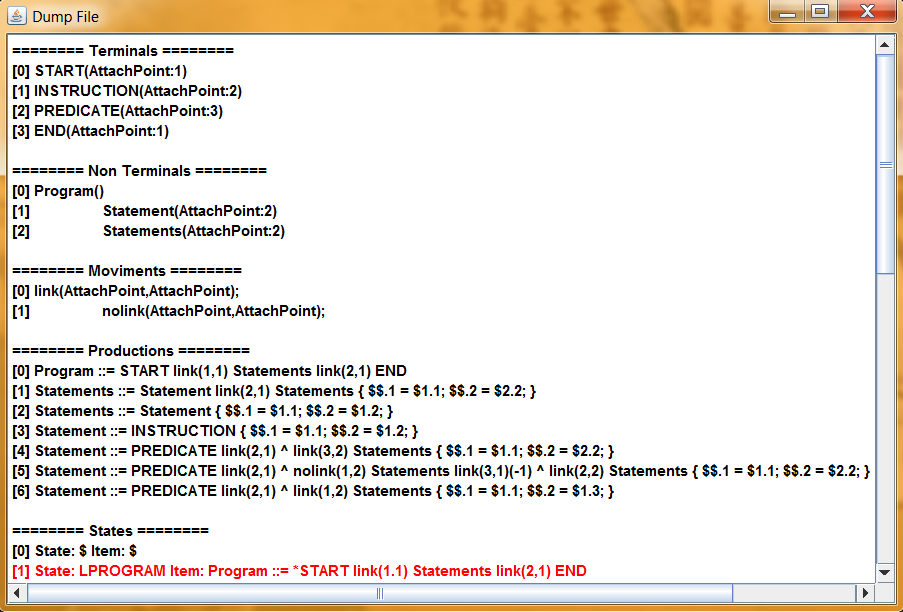
\includegraphics[height=250pt,width=330pt,scale=0.1]{files/DumpFile.png}}
	\caption{\textit{Informazioni sulla grammatica e sugli stati del parser}}
\end{figure}
\noindent La finestra in figura 7.8 viene utilizzata per rappresentare le informazioni inerenti alla grammatica che implementa il parser. Vengono descritti i terminali, i non-terminali, le produzioni, il simbolo iniziale (che corrisponde sempre alla prima produzione) e i vari item (stati) che vengono gestiti dal parser. Ogni volta che il parser esegue le operazioni di uno stato viene colorato di rosso.\par 
\begin{figure}[hbpb]\label{InsiemeR}
	\centering
	{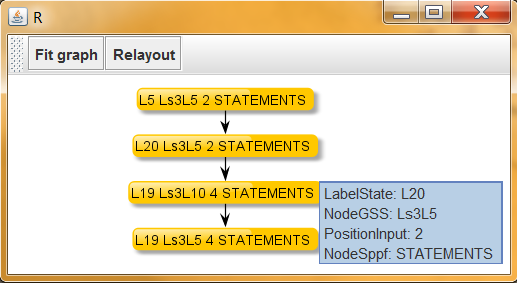
\includegraphics[height=130pt,width=250pt,scale=0.1]{files/InsiemeR.png}}
	\caption{\textit{Insieme R}}
\end{figure}
\noindent L'insieme R (fig. 7.9) viene rappresentato come una lista di nodi. Ogni nodo riporta le seguente informazioni: il nome dello stato, la posizione del simbolo da trovare, il nodo del GSS e il nodo dell'SPPF.